\subsection{Des algorithmes via un langage courant comme chez son pâtissier}
    \subsubsection{Manipulation de variables}
	\vspace{-0.75em}
	\begin{multicols}{2}
    \algoname{}
    Que renvoie l'algorithme suivant ?
    \bigskip
    \begin{myverb}
\(X\) prend la valeur \(6\).
\(X\) augmente de \(1\).
Renvoyer \(X\).
    \end{myverb}

    \switchcol

    \algoname{}
    Que renvoie l'algorithme suivant ?
    \bigskip
    \begin{myverb}
\(X\) prend la valeur \(2\).
\(X\) prend la valeur \(X+4\).
Renvoyer \(X\).
    \end{myverb}
\end{multicols}

\algorule

\begin{multicols}{2}
    \algoname{}
    Que renvoie l'algorithme suivant ?
    \bigskip
    \begin{myverb}
\(X\) prend la valeur \(10\).
\(X\) diminue de \(1\).
\(X\) prend la valeur \(X+3\).
\(X\) augmente de \(5\).
\(X\) prend la valeur \(100-X\).
Renvoyer \(X\).
    \end{myverb}

    \switchcol

    \algoname{}
    Que renvoie l'algorithme suivant ?
    \bigskip
    \begin{myverb}
\(X\) prend la valeur \(10\).
\(X\) prend la valeur \(X-4\).
\(X\) prend la valeur \(X+10\).
\(X\) prend la valeur \(X+3\).
\(X\) prend la valeur \(X-8\).
\(X\) prend la valeur \(199\,768-X\).
    \end{myverb}
\end{multicols}

\algorule

\begin{multicols}{2}
    \algoname{}
    Qu'affiche l'algorithme suivant ?
    \bigskip
    \begin{myverb}
\(X\) prend la valeur \(7\).
\(X\) prend la valeur \(X\times3\).
\(X\) prend la valeur \(X-11\).
Afficher \(X\).
    \end{myverb}

    \switchcol

    \algoname{}
    Qu'affiche l'algorithme suivant ?
    \bigskip
    \begin{myverb}
\(X\) prend la valeur \(7\).
\(X\) prend la valeur \(X-11\).
\(X\) prend la valeur \(X\times3\).
Afficher \(X\).
    \end{myverb}
\end{multicols}

% \algorule

\begin{multicols}{2}
    \algoname{}
    Est-il vrai que l'algorithme suivant affichera le nombre décimal $0,\!33333333333$ ?
    \bigskip
    \begin{myverb}
\(X\) prend la valeur \(9\).
\(X\) prend la valeur \(X-8\).
\(X\) prend la valeur \(\frac{X}{3}\).
Afficher \(X\).
    \end{myverb}

    \switchcol

    \algoname{}
    Est-il vrai que l'algorithme suivant affichera le nombre décimal $0,\!25$ ?
    \bigskip
    \begin{myverb}
\(X\) prend la valeur \(4\).
\(X\) prend la valeur \(-X\).
\(X\) prend la valeur \(X+5\).
\(X\) prend la valeur \(\frac{X}{4}\).
    \end{myverb}
\end{multicols} 

\subsubsection{Tester des situations}
	\vspace{-0.75em}
	\begin{multicols}{2}
    \algoname{}
    Qu'affiche l'algorithme ci-dessous lorsque $a=-1$ ?
    Même question pour $a=3$, puis pour $a=2$ ?
    \bigskip
    \begin{myverb}
Donnée
    Un réel \(a\).
Actions
    Si \(a\) est supérieur ou égal à \(2\) alors :
        Afficher \(a\sp{2}\).
    Sinon :
        Afficher \(a+2\).
    Fin du ou des test(s) Si
    \end{myverb}

    \switchcol

    \algoname{}
    Qu'affiche l'algorithme ci-dessous lorsque $a=-1$ ?
    Même question pour $a=3$, puis pour $a=2$ ?
    \bigskip
    \begin{myverb}
Donnée
    Un réel \(a\).
Actions
    Si a est supérieur ou égal à 2 alors :
        Afficher \(a\sp{2}\).
    Sinon si a est inférieur ou égal à \((-2)\) alors :
        Afficher \(a+2\).
    Fin du ou des test(s) Si
    \end{myverb}
\end{multicols}

\algorule

\begin{multicols}{2}
    \algoname{}
    Que renvoie l'algorithme ci-dessous lorsque $n=10$ ?
    Même question pour $n=7$ ?
    \bigskip
    \begin{myverb}
Donnée
    Un naturel \(n\).
Actions
    Si \(n\) est pair alors :
        \(n\) prend pour valeur le quotient de
        la division euclidienne de \(n\) par \(2\).
    Sinon :
        \(n\) prend pour valeur \(3n+1\).
    Fin du ou des test(s) Si
    Renvoyer \(n\).
    \end{myverb}

    \switchcol

    \algoname{}
    Cet algorithme renverra toujours la même chose que l'algorithme précédent n°11.
    Vrai ou faux ?
    \bigskip
    \begin{myverb}
Donnée
    Un naturel \(n\).
Actions
    Si \(n\) est pair alors :
        \(n\) prend pour valeur le quotient de
        la division euclidienne de \(n\) par \(2\).
    Sinon :
        \(n\) prend pour valeur \(3n+1\).
        Renvoyer \(n\).
    Fin du ou des test(s) Si
    \end{myverb}
\end{multicols}

\algorule

\begin{multicols}{2}
    \algoname{}
    Qu'affiche l'algorithme ci-dessous lorsque $n=11$, $n=33$, $n=4$, $n=70$, et enfin $n=25$ ?
    \bigskip
    \begin{myverb}
Donnée
    Un naturel \(n\).
Actions
    Si \(n\) est un multiple de \(2\) alors :
        \(n\) prend pour valeur \(\frac{n}{2}\).
    Sinon si \(n\) est un multiple de \(3\) alors :
        \(n\) prend pour valeur \(\frac{n}{3}\).
    Sinon si \(n\) est un multiple de \(5\) alors :
        \(n\) prend pour valeur \(\frac{n}{5}\).
    Sinon :
        \(n\) prend pour valeur \(0\).
    Fin du ou des test(s) Si
    Afficher \(n\) sous forme réduite.
    \end{myverb}

    \switchcol

    \algoname{}
    Qu'affiche l'algorithme ci-dessous lorsque $n=11$, $n=33$, $n=4$, $n=70$, et enfin $n=25$ ?
    \bigskip
    \begin{myverb}
Donnée
    Un naturel \(n\).
Actions
    Si \(n\) est un multiple de \(2\) alors :
        \(n\) prend pour valeur \(\frac{n}{2}\).
    Fin du ou des test(s) Si
    Si \(n\) est un multiple de \(3\) alors :
        \(n\) prend pour valeur \(\frac{n}{3}\).
    Fin du ou des test(s) Si
    Si \(n\) est un multiple de \(5\) alors :
        \(n\) prend pour valeur \(\frac{n}{5}\).
    Sinon :
        \(n\) prend pour valeur \(0\).
    Fin du ou des test(s) Si
    Afficher \(n\) sous forme réduite.
    \end{myverb}
\end{multicols}
 

\subsubsection{Répéter une action un nombre de fois \og connu \fg}
	\vspace{-0.75em}
	\begin{multicols}{2}
    \algoname{}
    Qu'affiche l'algorithme suivant ?
    \bigskip
    \begin{myverb}
Pour \(TEST\) un naturel allant de \(2\) 
à \(4\) faire :
    Afficher \(TEST\).
Fin de la boucle Pour
    \end{myverb}

    \switchcol

    \algoname{}
    Qu'affiche l'algorithme suivant ?
    \bigskip
    \begin{myverb}
Pour \(CONCENTRE\) un naturel pair allant
de \(3\) à \(12\) faire :
    Afficher \(CONCENTRE\).
Fin de la boucle Pour
    \end{myverb}
\end{multicols}

\algorule

\begin{multicols}{2}
    \algoname{}
    Qu'affiche l'algorithme ci-dessous pour $X=6$ ?
    \bigskip
    \begin{myverb}
Donnée
    Un réel \(X\).
Actions
    Afficher \(X\).
    Pour \(i\) un naturel allant de \(1\) à \(3\) faire :
        \(X\) prend la valeur \(X+1\).
    Fin de la boucle Pour
    \end{myverb}

    \switchcol

    \algoname{}
    Qu'affiche l'algorithme ci-dessous pour $X=6$ ?
    \bigskip
    \begin{myverb}
Donnée
    Un réel \(X\).
Actions
    Pour \(i\) un naturel allant de \(1\) à \(3\) faire :
        Afficher \(X\).
        \(X\) prend la valeur \(X+1\).
    Fin de la boucle Pour
    \end{myverb}
\end{multicols}

\algorule

\begin{multicols}{2}
    \algoname{}
    Qu'affiche l'algorithme ci-dessous pour $X=6$ ?
    \bigskip
    \begin{myverb}
Donnée
    Un réel \(X\).
Actions
    Pour \(i\) un naturel allant de \(1\) à \(3\) faire :
        \(X\) prend la valeur \(X+1\).
        Afficher \(X\).
    Fin de la boucle Pour
    \end{myverb}

    \switchcol

    \algoname{}
    Qu'affiche l'algorithme ci-dessous pour $X=6$ ?
    \bigskip
    \begin{myverb}
Donnée
    Un réel \(X\).
Actions
    Pour \(i\) un naturel allant de \(1\) à \(3\) faire :
        \(X\) prend la valeur \(X+1\).
    Fin de la boucle Pour
    Afficher \(X\).
    \end{myverb}
\end{multicols}

\algorule

\begin{multicols}{2}
    \algoname{}
    Qu'affiche l'algorithme ci-après lorsque $S=6$ ?
    \bigskip
    \begin{myverb}
Donnée
    Un réel \(S\).
Actions
    Pour \(k\) un naturel allant de \(1\) à \(3\) faire :
        \(S\) prend la valeur \(S+k\).
    Fin de la boucle Pour
    Afficher \(S\).
    \end{myverb}

    \switchcol

    \algoname{}
    Qu'affiche l'algorithme ci-après lorsque $S=11$ ?
    \bigskip
    \begin{myverb}
Donnée
    Un réel \(S\).
Actions
    Pour \(i\) un naturel allant de \(1\) à \(3\) faire :
        \(R\) est la valeur renvoyée par l'algorithme
        n°11 appliqué à \(S\) (voir la section 4.1.2).
        \(S\) prend la valeur \(R\).
    Fin de la boucle Pour
    Afficher \(S\).
    \end{myverb}
\end{multicols} 



\subsection{Certains algorithmes directement sous forme de diagrammes}

    Les diagrammes proposés en exercice dans cette section seront désignés par le néologisme \og algorigrammes \fg{}
    \footnote{
        Tous les diagrammes ont tous été réalisés avec le logiciel libre et gratuit
        LaTeXDraw que vous pourrez télécharger à l'adresse suivante :
        \url{http://latexdraw.sourceforge.net}.
    }. Nous n'utiliserons pas les conventions usuelles.

    \subsubsection{Utilisation de textes}
    Commençons par un cas simple qui devrait vous rappeler de bons ou mauvais souvenirs. Qu'affiche l'algorithme représenté par l'algorigramme ci-dessous lorsque $n=10$, $n=5$ puis $n=18$ ?
\begin{center}
	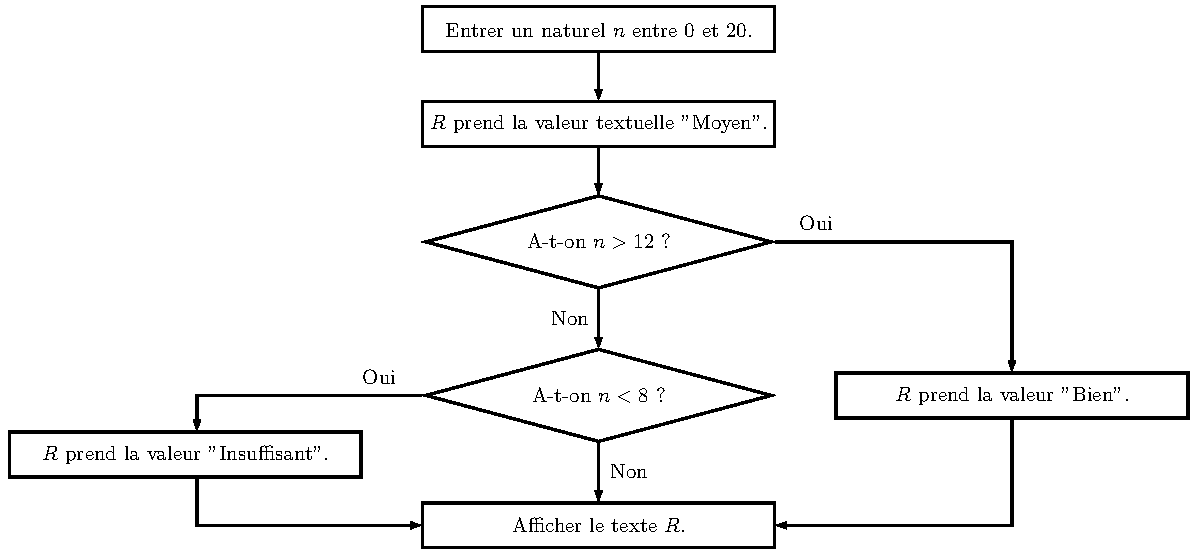
\includegraphics[width=1\textwidth]{reading/draw/text.pdf}
\end{center}


\subsubsection{Répéter une action un nombre de fois \og inconnu \fg}
    Considérons l'algorigramme ci-dessous.
\begin{center}
	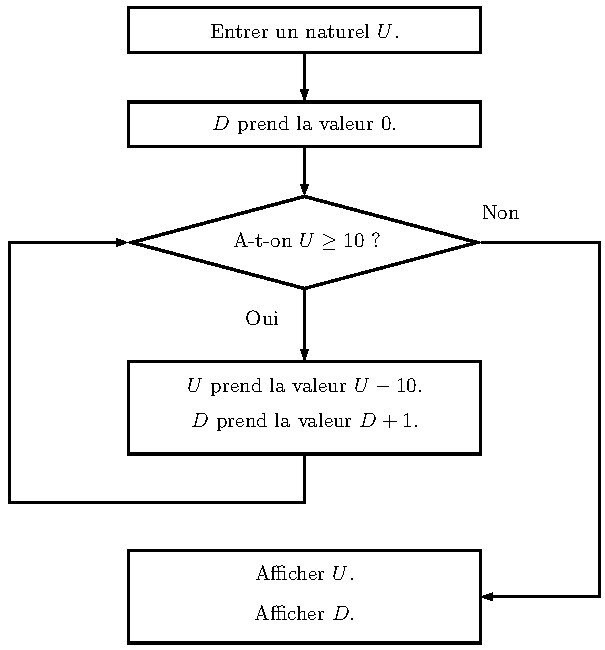
\includegraphics[width=0.5\textwidth]{reading/draw/while_loop.pdf}
\end{center}
Traduire cet algorigramme en langage naturel puis déterminer l'affichage obtenu lorsque $U = 43$.

\subsubsection{Répéter une action un nombre de fois \og connu \fg}
    \begin{multicols}{2}
    \algoname{}
    Qu'affiche l'algorithme suivant ?
    \bigskip
    \begin{myverb}
Pour \(TEST\) un naturel allant de \(2\) 
à \(4\) faire :
    Afficher \(TEST\).
Fin de la boucle Pour
    \end{myverb}

    \switchcol

    \algoname{}
    Qu'affiche l'algorithme suivant ?
    \bigskip
    \begin{myverb}
Pour \(CONCENTRE\) un naturel pair allant
de \(3\) à \(12\) faire :
    Afficher \(CONCENTRE\).
Fin de la boucle Pour
    \end{myverb}
\end{multicols}

\algorule

\begin{multicols}{2}
    \algoname{}
    Qu'affiche l'algorithme ci-dessous pour $X=6$ ?
    \bigskip
    \begin{myverb}
Donnée
    Un réel \(X\).
Actions
    Afficher \(X\).
    Pour \(i\) un naturel allant de \(1\) à \(3\) faire :
        \(X\) prend la valeur \(X+1\).
    Fin de la boucle Pour
    \end{myverb}

    \switchcol

    \algoname{}
    Qu'affiche l'algorithme ci-dessous pour $X=6$ ?
    \bigskip
    \begin{myverb}
Donnée
    Un réel \(X\).
Actions
    Pour \(i\) un naturel allant de \(1\) à \(3\) faire :
        Afficher \(X\).
        \(X\) prend la valeur \(X+1\).
    Fin de la boucle Pour
    \end{myverb}
\end{multicols}

\algorule

\begin{multicols}{2}
    \algoname{}
    Qu'affiche l'algorithme ci-dessous pour $X=6$ ?
    \bigskip
    \begin{myverb}
Donnée
    Un réel \(X\).
Actions
    Pour \(i\) un naturel allant de \(1\) à \(3\) faire :
        \(X\) prend la valeur \(X+1\).
        Afficher \(X\).
    Fin de la boucle Pour
    \end{myverb}

    \switchcol

    \algoname{}
    Qu'affiche l'algorithme ci-dessous pour $X=6$ ?
    \bigskip
    \begin{myverb}
Donnée
    Un réel \(X\).
Actions
    Pour \(i\) un naturel allant de \(1\) à \(3\) faire :
        \(X\) prend la valeur \(X+1\).
    Fin de la boucle Pour
    Afficher \(X\).
    \end{myverb}
\end{multicols}

\algorule

\begin{multicols}{2}
    \algoname{}
    Qu'affiche l'algorithme ci-après lorsque $S=6$ ?
    \bigskip
    \begin{myverb}
Donnée
    Un réel \(S\).
Actions
    Pour \(k\) un naturel allant de \(1\) à \(3\) faire :
        \(S\) prend la valeur \(S+k\).
    Fin de la boucle Pour
    Afficher \(S\).
    \end{myverb}

    \switchcol

    \algoname{}
    Qu'affiche l'algorithme ci-après lorsque $S=11$ ?
    \bigskip
    \begin{myverb}
Donnée
    Un réel \(S\).
Actions
    Pour \(i\) un naturel allant de \(1\) à \(3\) faire :
        \(R\) est la valeur renvoyée par l'algorithme
        n°11 appliqué à \(S\) (voir la section 4.1.2).
        \(S\) prend la valeur \(R\).
    Fin de la boucle Pour
    Afficher \(S\).
    \end{myverb}
\end{multicols}



\subsection{En utilisant un langage symbolique}
    \subsubsection{Est-ce efficace ?}
	Nous redonnons ci-dessous la version \og langage naturel \fg{} de l'algorithme n°14, puis nous proposons à côté une version symbolique de  cet algorithme. Repérez les conventions utilisées. On constate que l'écriture \og symbolique \fg{} est très économe en texte, et du coup il est très facile de la parcourir pour l'analyser.

\begin{multicols}{2}
    {\small\textbf{\textsc{[Algo.14]}}}
    \bigskip
    \begin{myverb}
Donnée
    Un naturel \(N\).
Actions
    Si \(N\) est un multiple de \(2\) alors :
        \(N\) prend pour valeur \(\frac{N}{2}\).
    Fin du ou des test(s) Si
    Si \(N\) est un multiple de \(3\) alors :
        \(N\) prend pour valeur \(\frac{N}{3}\).
    Fin du ou des test(s) Si
    Si \(N\) est un multiple de \(5\) alors :
        \(N\) prend pour valeur \(\frac{N}{5}\).
    Sinon :
        \(N\) prend pour valeur \(0\).
    Fin du ou des test(s) Si
    Afficher \(N\) sous forme réduite.
    \end{myverb}

    \switchcol

    {\small\textbf{\textsc{[Algo.14 "Symbolique"]}}}
    Ci-dessous, $k \, | \, n$ signifie que le naturel $k$ divise le naturel $n$.
    Par exemple, $3$ divise $15$ mais il ne divise pas $13$.
    \bigskip
    \begin{algo}
        \Data{$n \in \NN$}
        \Begin{
            \If{$2 \, | \, n$}{
                $n \leftarrow \frac{n}{2}$
            }
            \If{$3 \, | \, n$}{
                $n \leftarrow \frac{n}{3}$
            }
            \If{$5 \, | \, n$}{
                $n \leftarrow \frac{n}{5}$
            }
            \Print{$n$ sous forme réduite.}
        }
    \end{algo}
\end{multicols}






\subsubsection{Un retour en boucle}
	\begin{multicols}{2}
    \algoname{}
    Qu'affiche l'algorithme ci-dessous lorsque $n=6$ ?
    \bigskip
    \begin{algo}
        \Data{$n$ un naturel}
        \Begin{
            $F = 1$
            \\
            \For{$i = 1$ \KwTo $n$}{
                $F \leftarrow F \times i$
            }
            \Print{$F$}.
        }
    \end{algo}

    \switchcol

    \algoname{}
    Qu'affiche l'algorithme ci-dessous lorsque $x=6$ puis $x=12$ ?
    \bigskip
    \begin{algo}
        \Data{un réel $x$.}
        \Begin{
            \While{$x \leq 10$}{
                $x \leftarrow x + 1$
                \\
                \Print{$x$}.
            }
        }
    \end{algo}
\end{multicols}   
	

\subsubsection{Traduire en version symbolique}
	Donner une version symbolique des algorithmes n°9, n°10 et n°11. Faire de même avec les deux algorigrammes présentés dans les sections 4.2.1 et 4.2.2.   


\newpage

\subsection*{Annexe : Les algorigrammes ou la folie des grandeurs}
    Cette annexe utilise le logiciel LARP qui est gratuit depuis le 1\textsuperscript{er} Mars 2008, téléchargeable à l'adresse suivante \url{http://www.larp.marcolavoie.ca/fr/default.htm}, et qui malheureusement ne fonctionne que sous Windows\textsuperscript{\textcopyright}. 
LARP, qui est l'acronyme de Logiciel d'Algorithmes et de Résolution de Problèmes, permet au choix de taper des programmes ou bien d'utiliser des algorigrammes.
La seconde option permet de produire l'algorigramme ci-dessous qui propose une méthode de résolution dans $\RR$ d'une équation polynomiale du second degré
\footnote{
	Nul besoin de connaître cette théorie qui est généralement abordée en classe de première. L'idée ici est juste de comparer \og visuellement \fg{} différentes représentations d'un algorithme non simplistes.
}
où nous supposons implicitement que $a \neq  0$.

\begin{center}
	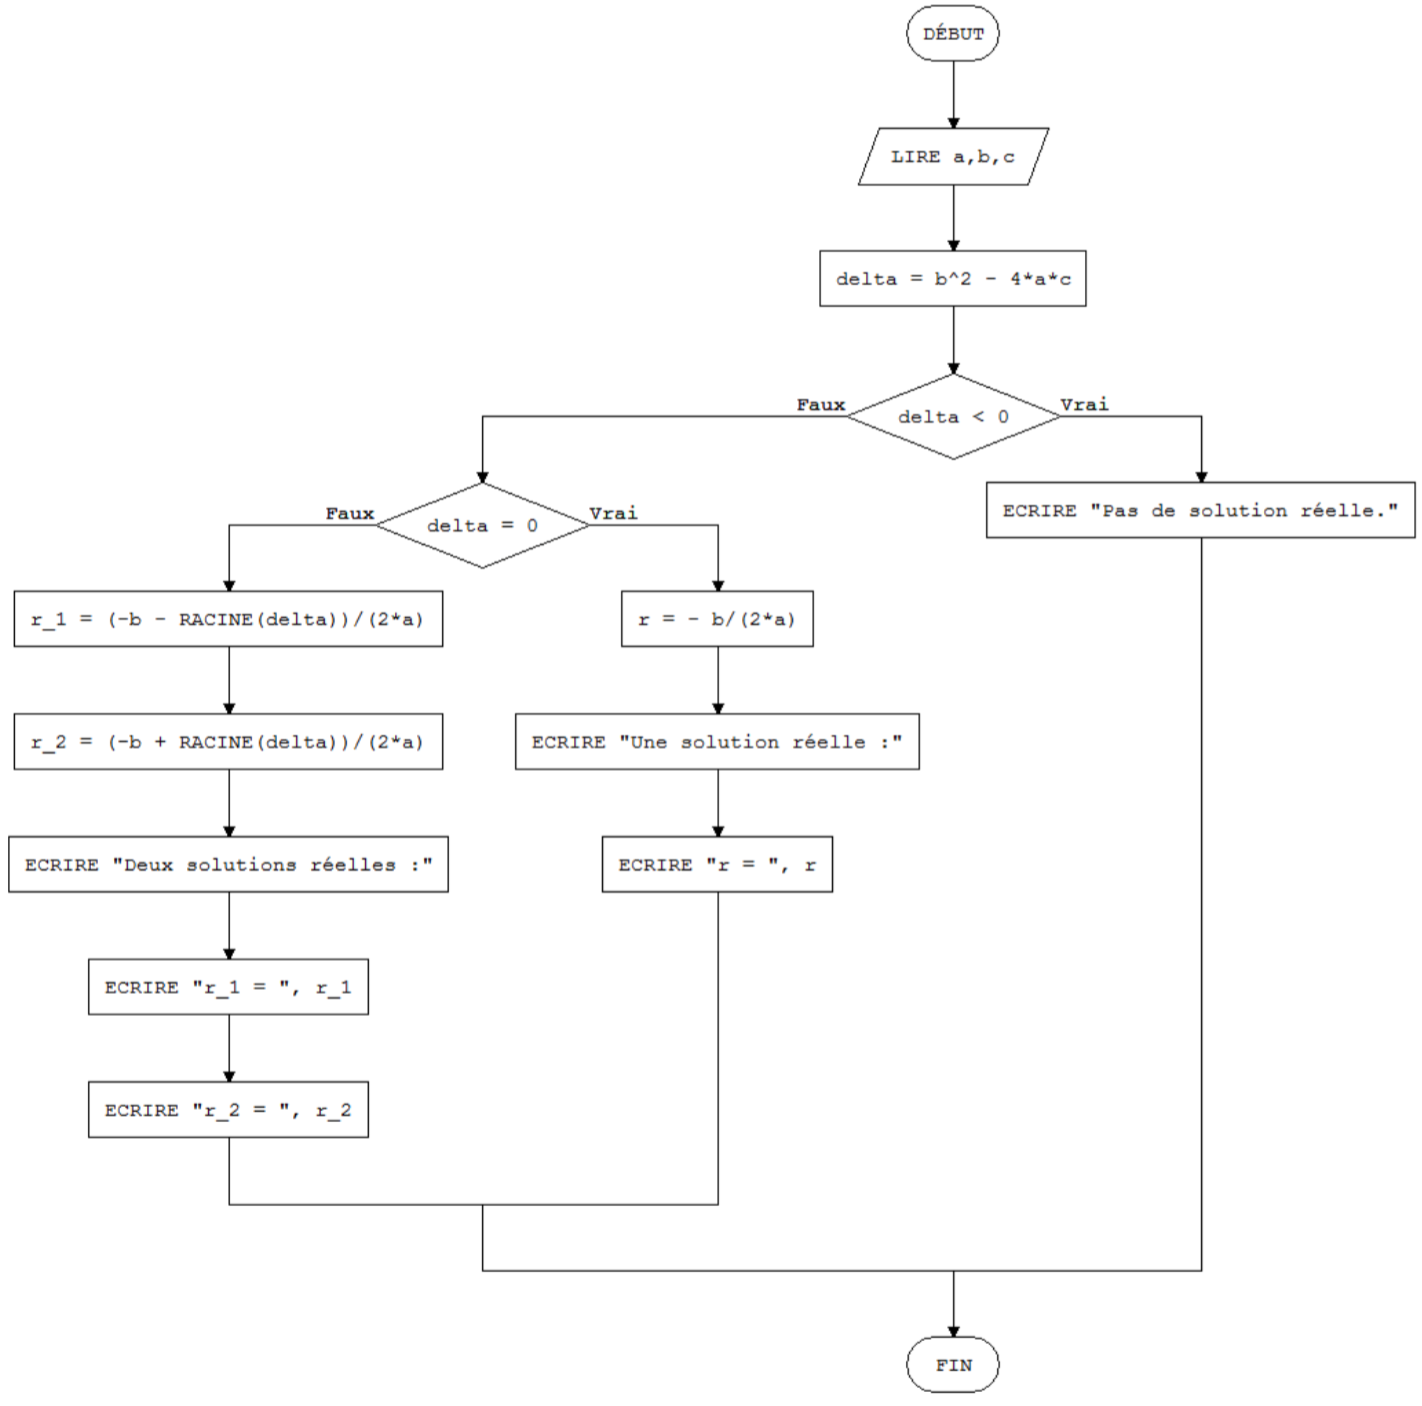
\includegraphics[width=1\textwidth]{reading/draw_limits/real_quadratic_equations.png}
\end{center}


LARP permet de produire directement une version \og programme \fg{} de l'algorigramme précédent. Nous obtenons ce qui suit où de nouveau nous supposons implicitement que $a \neq  0$.

\newpage

\begin{myverb}
DÉBUT
    LIRE a,b,c
    delta = b^2 - 4*a*c
    SI delta < 0 ALORS
        ECRIRE "Pas de solution réelle."
    SINON
        SI delta = 0 ALORS
            r = - b/(2*a)
            ECRIRE "Une solution réelle :"
            ECRIRE "r = ", r
        SINON
            r_1 = (-b - RACINE(delta))/(2*a)
            r_2 = (-b + RACINE(delta))/(2*a)
            ECRIRE "Deux solutions réelles :"
            ECRIRE "r_1 = ", r_1
            ECRIRE "r_2 = ", r_2
        FINSI
    FINSI
FIN

\end{myverb}
\bigskip

La comparaison des deux représentations précédentes montre qu'un algorigramme devient vite très encombrant. La version symbolique ci-après montre que l'on peut faire encore mieux.


\bigskip
\begin{algo}
    \Data{$(a , b , c) \in \RR^3$ où l'on suppose $a \neq  0$}
    \Begin{
	$\Delta = b^2 - 4 ac$ \\
        \eIf{$\Delta < 0$}{
		\Print{"Pas de solution réelle."}
        }{
		\eIf{$\Delta = 0$}{
			$r = \dfrac{-b}{2a}$ \\
			\vspace{0.5em}
			\Print{"Une solution réelle :"} \\
			\Print{"r = ", r} \\
        	}{
			$r_1 = \dfrac{-b - \sqrt{\Delta}}{2a}$
			et
			$r_2 = \dfrac{-b + \sqrt{\Delta}}{2a}$ \\
			\vspace{0.5em}
			\Print{"Deux solutions réelles :"} \\
			\Print{"$r_1$ = ", $r_1$} \\
			\Print{"$r_2$ = ", $r_2$} \\
		}
	}
    }
\end{algo}
\bigskip


En résumé, les algorigrammes sont un très bon outil quand l'on prend contact avec les algorithmes et la programmation mais ils montrent très vite leur limite quand on s'attaque à de \og vrais \fg{} problèmes.
